

\documentclass{article}
\usepackage[top=0cm, bottom=2cm, outer=0cm, inner=0cm,a4paper]{geometry}
\usepackage[pages=some]{background}
\usepackage{xcolor}
\usepackage{fontspec}
\usepackage{multicol}

\newcommand{\AwardEntry}[4]{
\begin{tabular}{ l l r }
  \textbf{\textcolor{materialPurple}{#1}}\hspace{20pt} & \textbf{#2} & {\small \textcolor{textLightGray}{#4}}\\
  	& \normalsize #3\\
\end{tabular}
\vspace*{10pt}
}


\newcommand{\ContactEntry}[2]{
	$\begin{array}{l}
	{\includegraphics[height=15pt]{#1}}
	\end{array}
	$ #2
}

\newcommand{\ExperienceEntry}[5]{
\begin{tabular}{  p{\dimexpr 0.15\linewidth-2\tabcolsep} 
                   p{\dimexpr 0.70\linewidth-2\tabcolsep}}
  \textbf{\textcolor{materialRedDark}{#1-}}\textbf{\textcolor{materialRed}{#2}}\hspace{20pt} & \textbf{#3}\\
  	& \normalsize #4\\
  	&{\small \textcolor{textLightGray}{#5}}
\end{tabular}
\vspace*{10pt}
}

\newcommand{\textBox}[1]{
\hspace*{7pt}
\begin{tabular}{  p{\dimexpr 0.97\linewidth-2\tabcolsep} }
  	{\normalsize #1}
\end{tabular}
\vspace*{10pt}
}

\newcommand{\EducationEntry}[5]{
\begin{tabular}{  p{\dimexpr 0.15\linewidth-2\tabcolsep} 
                   p{\dimexpr 0.70\linewidth-2\tabcolsep}}
  \textbf{\textcolor{materialBlueDark}{#1-}}\textbf{\textcolor{materialBlue}{#2}}\hspace{20pt} & \textbf{#3}\\
  	& \normalsize #4\\
  	&{\small \textcolor{textLightGray}{#5}}
\end{tabular}
\vspace*{10pt}
}

\definecolor{materialGreen} 	{RGB}{068,225,130}
\definecolor{materialGreenDark} {RGB}{029,184,090}
\definecolor{materialRed}   	{RGB}{218,068,049}
\definecolor{materialRedDark}   {RGB}{173,045,031}
\definecolor{materialPurple}   	{RGB}{153,039,176}
\definecolor{materialPurpleDark}{RGB}{088,022,099}
\definecolor{materialBlue}  	{RGB}{044,116,246}
\definecolor{materialBlueDark}  {RGB}{010,082,216}
\definecolor{materialYellow}	{RGB}{254,193,005}
\definecolor{materialYellowDark}{RGB}{194,147,001}
\definecolor{textGray}			{RGB}{070,070,070}
\definecolor{textLightGray}		{RGB}{140,140,140}

%Using font Roboto as main font for the document
\setmainfont{Roboto}

\backgroundsetup{
scale=1,
color=black,
opacity=1,
placement=top,
angle=0,
contents={%
  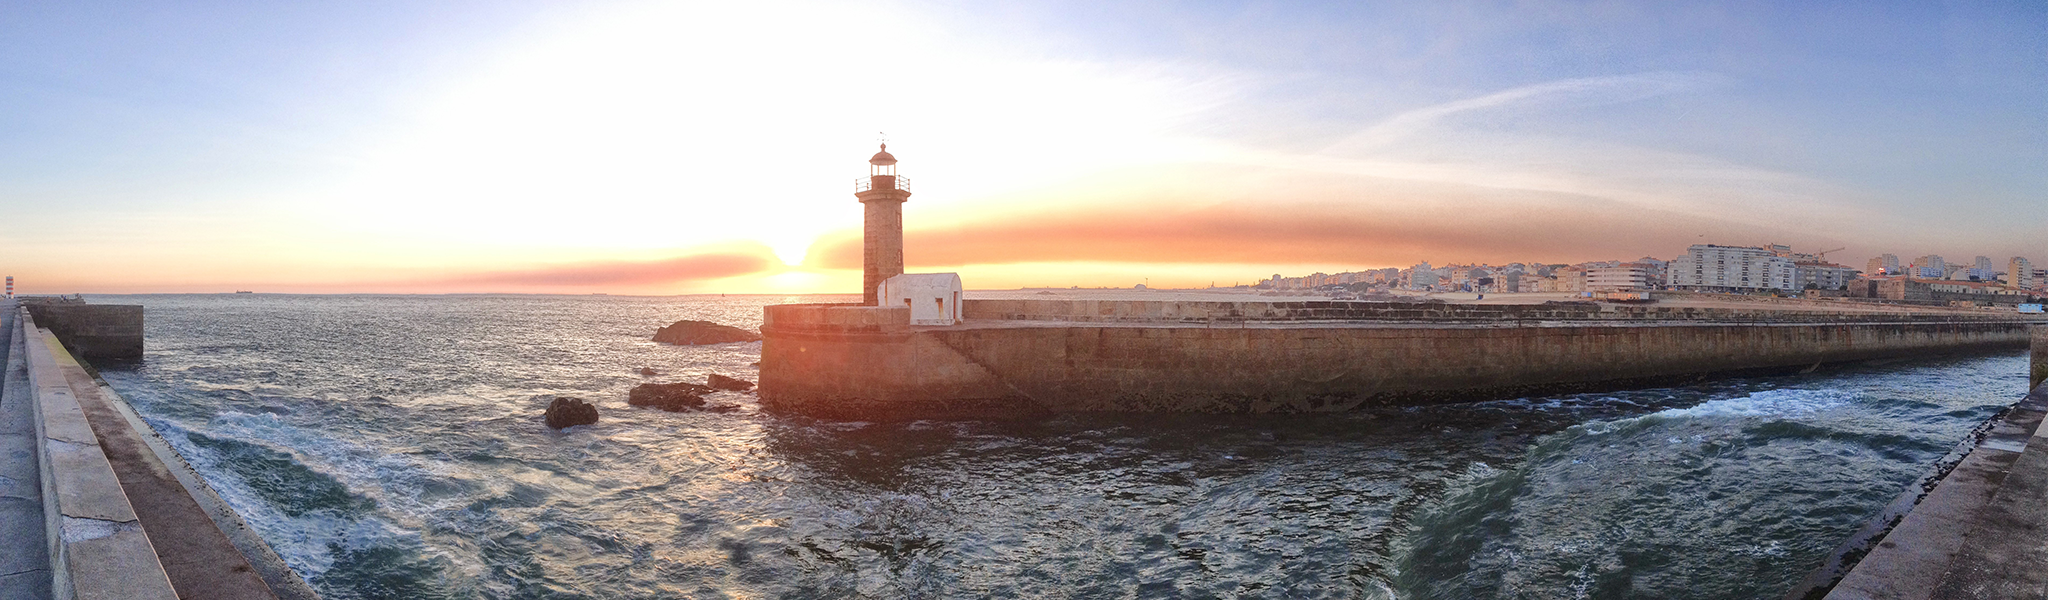
\includegraphics[width=\paperwidth,height=200pt]{images/pic}
  }%
}
\begin{document}
	\color{textGray}
	\pagenumbering{gobble}
	\vspace*{105pt} %spacing used to move the first and last name down
	\Huge
	\BgThispage
		\textcolor{white}{ImeKorisnika}

		\textcolor{white}{PrezimeKorisnika}
	\BgThispage
	\vspace*{20pt}
	%Include the main information from other tex files in order to get a better organization

	
\LARGE
\noindent\colorbox{materialGreen}
{\parbox[c][25pt][c]{\textwidth}{\hspace{15pt}\textcolor{white}{Contacts}}} %%Contacts separator

\begin{multicols}{2}

%%Contact Information
\large
%Add new or alter contact entries in this section by using the examples below
%for other contact information search the image folder for other icons
\ContactEntry{images/green/telephone1}{brojTelefona}

\ContactEntry{images/green/mail9}{mejlKorisnika}

\ContactEntry{images/green/links1}{linkVebsajta}

%\ContactEntry{images/green/linkedin2}{https://www.linkedin.com/in/yourname}
\columnbreak

\ContactEntry{images/green/house3}{UlicaIBroj}

\ContactEntry{images/green/map5}{mestoBoravka

\hspace*{25pt} Drzava}

\end{multicols}

	
\LARGE
\noindent\colorbox{materialRed}
{\parbox[c][25pt][c]{\textwidth}{\hspace{15pt}\textcolor{white}{Experience}}} %%Contacts separator

%%Contact Information
\large
\vspace*{10pt}
%Add new or alter education entries in this section by using the examples below
%\ExperienceEntry{starting year}{final year}{Position}{position description if applicable}{Place}
\ExperienceEntry{pocetak}{kraj}{Pozicija}{opisPosla.}{}

\vspace*{5pt}

	\LARGE
\noindent\colorbox{materialBlue}
{\parbox[c][25pt][c]{\textwidth}{\hspace{15pt}\textcolor{white}{Education}}} %%Contacts separator

%%Contact Information
\large
\vspace*{10pt}
%Add new or alter education entries in this section by using the examples below
%\EducationEntry{starting year}{final year}{Type of studies}{Studies description if applicable}{Place of studies}
\EducationEntry{2000}{2014}{Studies in something 1}{Studies description....}{}

\vspace*{5pt}
	
	\LARGE
\noindent\colorbox{materialYellow}
{\parbox[c][25pt][c]{\textwidth}{\hspace{15pt}\textcolor{white}{Interests}}} %%Contacts separator

%%Contact Information
\large
\vspace*{10pt}

\textcolor{materialYellow}{\textbf{Profes}}\textcolor{textGray}{\textbf{sional:}}\\
\textBox{
profesionalnaInteresovanja 
}\\

\textcolor{materialYellow}{\textbf{Pers}}\textcolor{textGray}{\textbf{onal:}}\\
\textBox{
privatnaInteresovanja
}\\
	
	
	
	%include awards information
	\LARGE
\noindent\colorbox{materialPurple}
{\parbox[c][25pt][c]{\textwidth}{\hspace{15pt}\textcolor{white}{Awards}}} %%Contacts separator

%%Contact Information
\large
\vspace*{5pt}

%Add new or alter education entries in this section by using the examples below
%\EducationEntry{starting year}{final year}{Type of studies}{Studies description if applicable}{Place of studies}
\AwardEntry{2000}{Studies in something 1}{Studies description....}{}

\vspace*{5pt}
\end{document}
